\begin{Problem}
	Wir definieren mit $S_n$ die Menge der bijektiven Abbildungen
	\[
	\sigma:\left\{ 1,\dots,n \right\} \to \left\{ 1,\dots,n \right\} 
	.\] 
	Dann ist bekannterweise $(S,\circ)$ mit
	\[
	\sigma_2\circ \sigma_1(i)=\sigma_2(\sigma_1(i))
	\]
	eine Gruppe. Wir führen für gewöhnlich eine Abbildungstabelle
	\[
		\sigma=\begin{pmatrix} 1 & 2 & \dots & n \\ i_1 & i_2 & \dots & i_n \end{pmatrix} \] 
		mit $i_1,\dots,i_n$ paarweise verschieden, um zu signalisieren $\sigma(k)=i_k$ f\"{u}r $k=1,\dots,n$.
		 \begin{parts}
			 \item Eine übliche Darstellung bei Elementen aus $S_n$ ist die Zyklenschreibweise. Ein Zyklus der Länge $k$ mit $k\le n$ hat die Form
				 \[
				 \sigma=(i_1,i_2,\dots, i_k)
				 \]
				 und signalisiert $i_1\to i_2, i_2\to i_3$, usw. $i_k\to i_1$ under $\sigma$. Ist die Zahl $i_j$ nicht im Zyklus vertreten, so wird sie unter $\sigma$ auf sich selbst abgebildet. Speziell f\"{u}r $k=1$ erhalten wir die Identität und schreiben
				 \[
				 \sigma=(1).\]
Geben Sie an, wie viele unterschiedliche Abbildungen $\sigma$ durch ein Zyklus der Länge $k$ realisiert werden können! Kann jedes Element in $S_3$ ($S_4$) als ein Zyklus geschriebeb werden?
\item Wir definieren die Menge der (Permutations-)Matrizen
	\[
		P_n:=\left\{ P\in \mathbb{K}^{n \times  n}: P=(e_{i_1},\dots,e_{i_n},\text{ mit }i\le i_k\le n\text{ und alle }i_k\text{ paarweise verschieden} \right\} 
	,\] 
	mit $e_i$ der $i$-te Einheitsvektor. Verifizieren Sie: $(P_n, \cdot)$ ist mit der herkömmlichen Matrixmultiplikation eine Gruppe! Bestimmen Sie weiterhin einen bijektiven Gruppenmorphismus
	\[
	\Phi:(S_n,\circ)\to(P_n,\cdot)
	,\] 
	sodass gilt
	\[
	\Phi(\sigma)e_i=s_j \iff\sigma(i)=j
	.\] 
	Beweisen Sie, dass sich jedes $P$ aus $P_n$ schreiben lässt als
	\[
		P=\prod_{k=1}^{n-1} V_{i_kj_k} 
	,\]
	mit $V_{ij}$ definiert wie in Lemma 5.56.
		\end{parts}
\end{Problem}
\begin{proof}
	\begin{parts}
	\item Es gibt $n!$ Möglichkeiten f\"{u}r eine Folge $(i_1i_2\dots i_k)$, aber wir können die zyklisch permutieren und $\sigma$ verändert sich nicht. Deswegen gibt es $n! / n = (n-1)!$ unterschiedliche Abbildungen, die durch ein Zyklus der Länge $k$ realisiert werden können.

		Ja, jedes Element in $S_3$ kann als ein Zyklus geschrieben werden. Das können wir explizit machen:
		\begin{align*}
			& (1) & (12) & & (23)\\
			& (13) & (132) & & (123)
		\end{align*}
		Weil wir $6$ Elemente haben, und $|S_3|=3! = 6$, haben wir alle Elemente.

		Das stimmt aber nicht f\"{u}r $S_4$. Sei
		\[
			\sigma=\begin{pmatrix} 1 & 2 & 3 & 4\\ 2 & 1 & 4 & 3 \end{pmatrix} 
		.\] 
		Falls es als Zyklus geschreiben werden kann, muss das Zyklus den Länge $4$ haben, weil $\sigma(i)\neq i$ f\"{u}r alle $i$. Wir fangen obdA mit $1$ an. Dann ist das Zyklus $(12\dots)$. Aber weil $\sigma(2)=1$, hört das Zyklus auf, und $\dots=\varnothing$. Dann ist das Zyklus nicht mit Länge 4. 
	\item Sei $A,B\in P_n$ beliebige Elemente von $P_n$,
		\begin{align*}
			A=&(e_{i_1},e_{i_2},\dots, e_{i_n})\\
			B=&(e_{j_1},e_{j_2},\dots, e_{j_n})
		\end{align*}
		\begin{enumerate}[label=(\roman*)]
			\item $G$ ist abgeschlossen: Wir betrachten $ABe_k$ f\"{u}r $k$ beliebig.
				\[
					ABe_k=Ae_{j_k}=e_{i_{j_k}}
				,\]
				also
				\[
					AB=(e_{i_{j_1}},e_{i_{j_2}},\dots,e_{i_{j_n}})\in P_n
				.\] 
				Das $i_{j_k}$ paarweise verscheiden sind folgt daraus, dass $j_k$ alle paarweise verscheiden sind.
			\item Neutrales element: Wir wissen aus der linearen Algebra, dass
				 \[
				1_n=(e_1,e_2,\dots, e_n)\in P_n
				\]
				das neutrales Element ist.
			\item Assoziativität: Wir wissen auch, dass Matrizmultiplikation assoziativ ist.
			\item Existenz des Inverses: Sei jetzt $p_k$, sodass $i_{p_k}=k$. 
				\begin{tcolorbox}[title=Bemerkung]
					Man kann $i,p: \left\{ 1,\dots,n \right\} \to \left\{ 1,\dots,n \right\} $ interpretieren. Dann ist $i$ eine bijektive Abbildung, und das Existenz einer inversen Abbildung $p$ folgt daraus. Deswegen ist unsere Entscheidung immer möglich.
				\end{tcolorbox}
				Wir betrachten $A(e_{p_1},e_{p_2},\dots, e_{p_n})$, und dafür die Wirkung der Abbildung auf einem beliebigen Basiselement $e_k$: 
\[
	A(e_{p_1},e_{p_2},\dots,e_{p_n})e_k=Ae_{p_k}=e_{i_{p_k}}=e_k
.\] 
		\end{enumerate}
	\item Sei $i$ eine bijektive Abbildung $\left\{ 1,\dots,n \right\}\to \left\{ 1,\dots,n \right\} $. Wir schreiben $i_k$ oder $i(k)$ als das Bild von $k$. Wir vermuten, dass die gewünschte Homomorphismus
		\[
		\Phi:i\to (e_{i_1},e_{i_2},\dots e_{i_n})
		\] 
		ist.
		\begin{enumerate}[label=(\roman*)]
			\item $\Phi(\sigma)e_j=e_{\sigma_j}$, also  $\Phi(\sigma)e_i=s_j\iff \sigma(i)=j$.
			\item Injektiv: Sei $\sigma,\sigma' \in S_n$, $\sigma\neq \sigma'$, insbesondere gilt $\sigma(i)\neq \sigma'(i)$. Es gilt dann
				 \begin{center}
					 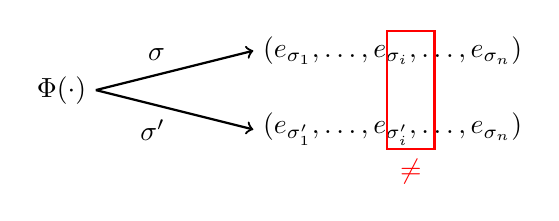
\begin{tikzpicture}[xscale=2,yscale=0.5]
						\draw (0,0) node[anchor=east] {$\Phi(\cdot)$};
						\draw[thick,->] (0,0) -- (1,1);
						\draw[thick,->] (0,0) -- (1,-1);
						\draw (1,1) node[anchor=west] {$(e_{\sigma_1},\dots,e_{\sigma_i},\dots,e_{\sigma_n})$};
						\draw (1,-1) node[anchor=west] {$(e_{\sigma'_1},\dots, e_{\sigma'_i},\dots,e_{\sigma_n})$};
						\draw (0.5,0.5) node[anchor=south east] {$\sigma$};
						\draw (0.5,-0.5) node[anchor=north east] {$\sigma'$};
						\draw[red,thick] (1.85,-1.5) rectangle (2.15,1.5);
						\draw[red] (2,-1.5) node[anchor=north] {$\neq$};
					\end{tikzpicture}
				\end{center}
				also $\Phi(\sigma)\neq \Phi(\sigma')$.
			\item Surjektiv: Sei $M=(e_{i_1},e_{i_2},\dots,e_{i_n}$. Wie im letzten Teilaufgabe können wir eine Abbildung $i(k)=i_k$ definieren, und $\Phi(i)=M$.
			\item Homomorphismusgesetz: Es ist zu zeigen, f\"{u}r $i,j\in S_n$ und 
				\begin{align*}
					M_1=&(e_{i_1},e_{i_2},\dots, e_{i_n})=\Phi(i)\\
					M_2=&(e_{j_1},e_{j_2},\dots,e_{j_n})=\Phi(j),
				\end{align*}
				dass
				 \[
				\Phi(i \circ j)(e_k)=M_1M_2e_k
				\] 
				f\"{u}r alle $k$ gilt. Per Definition ist
				\[
					\Phi(i\circ j)e_k=e_{i(j(k))}=e_{i_{j_k}}
				.\] 
				Es gilt auch
				\[
					M_1M_2e_k=M_1e_{j(k)}=e_{i(j(k))}=e_{i_{j_k}}
				.\] 
		\end{enumerate}
	\item Es gilt
		\[
			\Phi((ij))=V_{ij}
		\]
		per die vorherige Definition. Dann ist die Behauptung klar. Sei $P\in P_n$
		\begin{enumerate}[label=(\roman*)]
			\item Weil $\Phi$ bijektiv ist, ist $P=\Phi(\sigma)$ f\"{u}r eine $\sigma \in S_n$. 
			\item $\sigma$ kann als Produkt von $n-1$ Transpositionen dargestellt werden (wenn weniger als $n-1$, können wir $\text{id}$ hinzufügen), z.B. $\sigma=(a_1b_1)(a_2b_2)\dots(a_{n-1}b_{n-1})$. 
			\item Das Bild von ein Transposition ist ein Matriz $V_{ij}$. 
			\item Dann ist
				\begin{align*}
					\Phi(\sigma)=&\Phi((a_1b_1))\Phi((a_2b_2))\dots\Phi(a_{n-1}b_{n-1})\\
					=& V_{a_1b_1}V_{a_2b_2}\dots V_{a_{n-1}b_{n-1}}\\
					=&P.\qedhere
				\end{align*}
		\end{enumerate}
	\end{parts}
\end{proof}
\begin{Problem}
	Gegeben sei die Permutation
	\[
		S_9\ni \sigma =\begin{pmatrix} 1 & 2 & 3 & 4 & 5 & 6 & 7 & 8 & 9\\2 & 4 & 3 & 9 & 7 & 6 & 8 & 1 & 5 \end{pmatrix} 
	.\] 
	\begin{parts}
	\item Stellen sie $\sigma$ als Produkt von Transpositionen dar.
	\item Berechnen Sie das Signum von $\sigma$.
	\end{parts}
\end{Problem}
\begin{proof}
	\begin{parts}
	\item Zuerst berechnen wir die disjunkter Zyklus
		\begin{align*}
			Z_1=&(1249578)\\
			Z_2=&(6)\\
			Z_3=&(3)
		\end{align*}
		Dann haben wir
		\[
		\sigma=(18)(17)(15)(19)(14)(12)
		.\] 
		\begin{tcolorbox}[title=Begründung]
			Es gilt, f\"{u}r ein Zyklus
			\[
				(a_1a_2\dots a_n)=\underbrace{(a_1a_n)(a_1a_{n-1})\dots (a_1a_2)}_{\sigma'}
			.\] 
			Wir betrachten zuerst $\sigma'(a_1)$. Dann ist $(a_1a_2)a_1=a_2$. $a_2$ kommt nie wieder vor, also $\sigma'(a_1)=a_2$. Dann betrachten wir $a_k$, $k\neq 1$. Wir haben $(a_1a_k)a_k=a_1$. $a_1$ kommt sofort wieder vor, und ist $(a_1a_{k+1})a_1=a_{k+1}$. $a_{k+1}$ kommt nicht wieder vor, also $\sigma'(a_k)=a_{k+1}$.
		\end{tcolorbox}
	\item Wir haben
		\[
			\text{sgn}(\sigma)=\text{sgn}((18))\text{sgn}((17))\dots\text{sgn}((12))=(-1)^6=1
		.\qedhere\] 
	\end{parts}
\end{proof}
\begin{Problem}
	Sei $n\in \N$ mit $n\ge 2$. Eine Matrix  $A\in M_n(\R)$ heißt \emph{symmetrisch} bzw. \emph{antisymmetrisch}, wenn $A^T=A$ bzw. $A^T=-A$ gilt. Seien $\text{SM}_n(\R)$ bzw. $\text{AS}_n(\R)$ die Untermengen von $M_n(\R)$, die aus allen symmetrischen bzw. antisymmetrischen Matrizen bestehen.
	\begin{parts}
	\item Zeigen Sie, dass $\text{SM}_n(\R), \text{AS}_n(\R)$ Untervektorr\"{a}ume von $M_n(\R)$ sind.
	\item Zeigen Sie, dass
		\[
			A^T+A\in \text{SM}_n(\R), \qquad A-A^T\in \text{AS}_n(\R), \qquad \forall A\in M_n(\R)
		.\] 
		Folgern Sie, dass $M_n(\R)=\text{SM}_n(\R)\oplus \text{AS}_n(\R)$.
	\item Bestimmen Sie $\text{dim}(\text{SM}_n(\R))$ und $\text{dim}(\text{AS}_n(\R))$.
	\item Seien $A,B\in \text{AS}_n(\R)$ asymmetrische Matrizen. Zeigen Sie, dass der \emph{Kommutator} $[A,B]:=AB-BA$ wieder antisymmetrisch ist.
	\end{parts}
\end{Problem}
\begin{proof}
	\begin{parts}
	\item Sei $M,N\in \text{SM}_n(\R)$, und $a,b\in \R$. Es gilt
		\[
			(aM)^T=aM^T=aM
		,\]
		also $aM\in\text{SM}_n(\R)$. Es gilt auch
		\[
			(aM+bN)^T=aM^T+bN^T=aM+bN
		,\]
		also $aM+bN\in\text{SM}_n(\R)$.

		Sei jetzt $M,N\in\text{AS}_n(\R)$. Ähnlich folgt
		\[
			(aM)^T=aM^T=a(-M)=-aM
		,\] 
		und
		\[
			(aM+bN)^T=aM^T+bN^T=a(-M)+b(-N)=-(aM+bN)
		\]
		also $\text{SM}_n(\R)$ und $\text{AS}_n(\R)$ sind Untervektorräume.
	\item Es gilt
		\begin{align*}
			(A+A^T)^T=&A^T+(A^T)^T\\
			=& A^T+A=A+A^T\\
			(A-A^T)^T=&A^T-(A^T)^T\\
			=&A^T-A=-(A-A^T)
		\end{align*}
		F\"{u}r alle $A\in M_n(\R)$ gilt
		\[
			A=\frac{1}{2}(\underbrace{A+A^T}_{\in \text{SM}_n(\R)}+\underbrace{A-A^T}_{\in\text{AS}_n(\R)})
		,\] 
		also $M_n(\R)=\text{SM}_n(\R)\oplus \text{AS}_n(\R)$. 
	\item In ein Matriz gibt es genau $n \times n$ freie Parameter. Aber f\"{u}r symmetrische Matrizen haben wir $M_{xy}=M_{yx}$, also wir haben nur
		\[
		\sum_{i=1}^{n} i=\frac{n(n+1)}{2}
		\]
		freie Parameter in $\text{SM}_n(\R)$. F\"{u}r die antisymmetrischen Matrizen gilt eine ähnliche Argument, aber die Elemente auf dem Diagonal müssen $0$ sein. Wir haben daher nur
		\[
		\sum_{i=0}^{n-1} i=\frac{n(n-1)}{2}
		\]
		freie Parameter, also
		\begin{align*}
			\text{dim}(\text{SM}_n(\R))=&\frac{n(n+1)}{2}\\
			\text{dim}(\text{AS}_n(\R))=&\frac{n(n-1)}{2}
		\end{align*}
	\item Es gilt
		\begin{align*}
			[A,B]^T=&(AB-BA)^T\\
			=&(AB)^T-(BA)^T\\
			=&B^TA^T-A^TB^T\\
			=&(-B)(-A)-(-A)(-B)\\
			=&BA-AB\\
			=&-(AB-BA)
		\end{align*}
		also $[A,B]$ ist antisymmetrisch.\qedhere
	\end{parts}
\end{proof}
\begin{Problem}
	Gegeben sind die Matrizen $A(t)=\begin{pmatrix} 1 & 1 & 1\\1 & t^2 & 1\\t & 1 & 1 \end{pmatrix} $ und $B(t)=\begin{pmatrix} 1 & t & 0 \\ 0 & -1 & 1-t \\ 2 & 0 & t \end{pmatrix}, A,B\in \R^{3\times 3}, t\in \R$.
	\begin{parts}
	\item Bestimmen Sie $\text{rang}(A(t))$ und $\text{rang}(B(t))$ in Abhängigkeit von $t$.
	\item Berechnen Sie die Inversen $(A(0))^{-1}$ und $(B(1))^{-1}$.
	\end{parts}
\end{Problem}
\begin{proof}
	\begin{parts}
	\item Wir verwenden das Gauß-Algorithisums
		\begin{gather*}
			\left(
\begin{array}{ccc}
 1 & 1 & 1 \\
 1 & t^2 & 1 \\
 t & 1 & 1 \\
\end{array}
\right) \xrightarrow{R_2-R_1} \left(
\begin{array}{ccc}
 1 & 1 & 1 \\
 0 & t^2-1 & 0 \\
 t & 1 & 1 \\
\end{array}
\right) \xrightarrow{R_1\times t} \\\left(
\begin{array}{ccc}
 t & t & t \\
 0 & t^2-1 & 0 \\
 t & 1 & 1 \\
\end{array}
\right) \xrightarrow{R_3-R_1} \left(
\begin{array}{ccc}
 t & t & t \\
 0 & t^2-1 & 0 \\
 0 & 1-t & 1-t \\
\end{array}
\right) \xrightarrow{R_3\times t+1} \\\left(
\begin{array}{ccc}
 t & t & t \\
 0 & t^2-1 & 0 \\
 0 & 1-t^2 & 1-t^2 \\
\end{array}
\right) \xrightarrow{R_3+R_2} \left(
\begin{array}{ccc}
 t & t & t \\
 0 & t^2-1 & 0 \\
 0 & 0 & 1-t^2 \\
\end{array}
\right)
		\end{gather*}
F\"{u}r $t\neq 0, t^2-1\neq 0$, also $t\not\in \left\{ -1,0, 1\right\} $, ist es offenbar, $\text{rang}(A(t))=3$ ist.

F\"{u}r $t=\pm 1$ ist $A=\begin{pmatrix} 1 & 1 & 1 \\ 1 & 1 & 1 \\ 1 & 1 & 1 \end{pmatrix} $, also $Ae_1=Ae_2=Ae_3\neq 0$. Daraus folgt, dass $\text{rang}(A(\pm 1))=1$.

Obwohl es vom Gauß-Algorithismus so aussieht, dass  $\text{rang}(A(0))\neq 3$, ist eigentlich $\text{rang}(A(0))=3$. Wenn $t=0$ gilt
\[
	A(0)=\begin{pmatrix} 1 & 1 & 1 \\ 1 & 0 & 1 \\ 0 & 1 & 1 \end{pmatrix} 
.\] 
Man beachte dann, dass
\begin{align*}
	A(e_3-e_1)=&(0,0,1)^T\\
	A(e_3-e_2)=&(0,1,0)^T\\
	A(e_1+e_2-e_3)=&(1,0,0)^T
\end{align*}
Weil wir jede Basiselement erreichen können, können wir also jedes Element $v\in \R^3$ erreichen. Deswegen gilt $\text{rang}(A(0))=3$. Zusammenfassung:
\[
	\text{rang}(A(t))=\begin{cases}
		1 & t=\pm 1,\\
		3 & \text{sonst.}
	\end{cases}
.\] 

Wir machen etwas ähnliches für $B$ :
\begin{gather*}
	\left(
\begin{array}{ccc}
 1 & t & 0 \\
 0 & -1 & 1-t \\
 2 & 0 & t \\
\end{array}
\right) \xrightarrow{R_3-2R_1} \left(
\begin{array}{ccc}
 1 & t & 0 \\
 0 & -1 & 1-t \\
 0 & -2 t & t \\
\end{array}
\right) \xrightarrow{R_2\times 2 t}\\ \left(
\begin{array}{ccc}
 1 & t & 0 \\
 0 & -2 t & -2 (t-1) t \\
 0 & -2 t & t \\
\end{array}
\right) \xrightarrow{R_3-R_2} \left(
\begin{array}{ccc}
 1 & t & 0 \\
 0 & -2 t & -2 (t-1) t \\
 0 & 0 & t (2 t-1) \\
\end{array}
\right) 
\end{gather*}
Offenbar gilt, dass wenn $t\neq 0$ und $t\neq 1 / 2$, ist $\text{rang}(B(t))=3$. Wenn $t= 1 /2$, ist die Matriz
\[
	\begin{pmatrix}  1 & 1 / 2 & 0 \\ 0 & -1 & -1 / 2 \\ 0 & 0 & 0 \end{pmatrix} 
,\] 
also $\text{rang}(B(1 / 2))=2$. Wenn $t=0$ dürfen wir das Ergebnis des Gauß-Algorithismuses nicht direkt nutzen, weil wir durch $2t$ multiplizieren haben. Stattdessen schreiben wir
\[
	B(0)=\begin{pmatrix} 1 & 0 & 0 \\ 0 & -1 & 1\\ 2 & 0 & 0 \end{pmatrix} 
.\] 
Jetzt ist es klar, dass
\[
	\text{im}(B(0))=\text{span}\left\{ \begin{pmatrix} 1 \\ 0 \\ 2 \end{pmatrix} , \begin{pmatrix}  0 \\ 1 \\ 0\end{pmatrix}  \right\} 
,\]
also $\text{rang}(B(0))=2$.
\item Wir haben
	\[
		A(0)=\begin{pmatrix}  1 & 1 & 1 \\ 1 & 0 & 1 \\ 0 & 1 & 1 \end{pmatrix} \qquad B(1)=\begin{pmatrix} 1 & 1 & 0 \\ 0 & -1 & 0 \\ 1 & 0 & 1 \end{pmatrix} 
	.\] 
Dann
\begin{gather*}
	\left(
\begin{array}{ccc|ccc}
 1 & 1 & 1 & 1 & 0 & 0 \\
 1 & 0 & 1 & 0 & 1 & 0 \\
 0 & 1 & 1 & 0 & 0 & 1 \\
\end{array}
\right) \xrightarrow{R_2-R_1} \left(
\begin{array}{ccc|ccc}
 1 & 1 & 1 & 1 & 0 & 0 \\
 0 & -1 & 0 & -1 & 1 & 0 \\
 0 & 1 & 1 & 0 & 0 & 1 \\
\end{array}
\right) \xrightarrow{R_3+R_2} \\\left(
\begin{array}{ccc|ccc}
 1 & 1 & 1 & 1 & 0 & 0 \\
 0 & -1 & 0 & -1 & 1 & 0 \\
 0 & 0 & 1 & -1 & 1 & 1 \\
\end{array}
\right) \xrightarrow{R_1+R_2} \left(
\begin{array}{ccc|ccc}
 1 & 0 & 1 & 0 & 1 & 0 \\
 0 & -1 & 0 & -1 & 1 & 0 \\
 0 & 0 & 1 & -1 & 1 & 1 \\
\end{array}
\right) \xrightarrow{R_1-R_3} \\\left(
\begin{array}{ccc|ccc}
 1 & 0 & 0 & 1 & 0 & -1 \\
 0 & -1 & 0 & -1 & 1 & 0 \\
 0 & 0 & 1 & -1 & 1 & 1 \\
\end{array}
\right) \xrightarrow{R_2\times -1} \left(
\begin{array}{ccc|ccc}
 1 & 0 & 0 & 1 & 0 & -1 \\
 0 & 1 & 0 & 1 & -1 & 0 \\
 0 & 0 & 1 & -1 & 1 & 1 \\
\end{array}
\right)
\end{gather*}
		Also $(A(0))^{-1}=\begin{pmatrix} 1 & 0 & -1 \\ 1 & -1 & 0 \\ -1 & 1 & 1 \end{pmatrix} $. Es gilt auch
		\begin{gather*}
			\left(
\begin{array}{ccc|ccc}
 1 & 1 & 0 & 1 & 0 & 0 \\
 0 & -1 & 0 & 0 & 1 & 0 \\
 1 & 0 & 1 & 0 & 0 & 1 \\
\end{array}
\right) \xrightarrow{R_3-R_1} \left(
\begin{array}{ccc|ccc}
 1 & 1 & 0 & 1 & 0 & 0 \\
 0 & -1 & 0 & 0 & 1 & 0 \\
 0 & -1 & 1 & -1 & 0 & 1 \\
\end{array}
\right) \xrightarrow{R_3-R_2} \\\left(
\begin{array}{ccc|ccc}
 1 & 1 & 0 & 1 & 0 & 0 \\
 0 & -1 & 0 & 0 & 1 & 0 \\
 0 & 0 & 1 & -1 & -1 & 1 \\
\end{array}
\right) \xrightarrow{R_1+R_2} \left(
\begin{array}{ccc|ccc}
 1 & 0 & 0 & 1 & 1 & 0 \\
 0 & -1 & 0 & 0 & 1 & 0 \\
 0 & 0 & 1 & -1 & -1 & 1 \\
\end{array}
\right) \xrightarrow{R_2\times -1} \\\left(
\begin{array}{ccc|ccc}
 1 & 0 & 0 & 1 & 1 & 0 \\
 0 & 1 & 0 & 0 & -1 & 0 \\
 0 & 0 & 1 & -1 & -1 & 1 \\
\end{array}
\right)
		\end{gather*}
		also
		\[
			(B(1))^{-1}=\begin{pmatrix} 1 & 1 & 0\\0 & -1 & 0 \\ -1 & -1 & 1 \end{pmatrix} 
		.\qedhere\] 
	\end{parts}
\end{proof}
